%% principal.tex, abntex-based v-1.9.6 laurocesar
%% Copyright 2012-2016 by abnTeX2 group at http://www.abntex.net.br/ 
%% Copyright 2016 by Ygor Amaral at http://www.ygoramaral.com
%%
%% This work may be distributed and/or modified under the
%% conditions of the LaTeX Project Public License, either version 1.3
%% of this license or (at your option) any later version.
%% The latest version of this license is in
%%   http://www.latex-project.org/lppl.txt
%% and version 1.3 or later is part of all distributions of LaTeX
%% version 2005/12/01 or later.
%%
%% This work has the LPPL maintenance status `maintained'.
%% 

% ---------------------------------------------------------------------------------
% ---------------------------------------------------------------------------------
% Modelo de PCC (Monografia) para o curso de Sistemas de Informação da UFRPE/UAST.
% Baseado no abnTeX2 que possui conformidade com diversas normas da ABNT.
% ---------------------------------------------------------------------------------
% ---------------------------------------------------------------------------------

\documentclass[
	% -- opções da classe memoir --
	12pt,				% tamanho da fonte
	openright,			% capítulos começam em pág ímpar (insere página vazia caso preciso)
	oneside,			% twoside para impressão em recto e verso. Oposto a oneside
	a4paper,			% tamanho do papel. 
	sumario=tradicional, % abnt-6027-2012 ou tradicional
	%sumario=abnt-6027-2012, % abnt-6027-2012 ou tradicional
	% -- opções da classe abntex2 --
	%chapter=TITLE,		% títulos de capítulos convertidos em letras maiúsculas
	%section=TITLE,		% títulos de seções convertidos em letras maiúsculas
	%subsection=TITLE,	% títulos de subseções convertidos em letras maiúsculas
	%subsubsection=TITLE,% títulos de subsubseções convertidos em letras maiúsculas
	% -- opções do pacote babel --
	english,			% idioma adicional para hifenização
	french,				% idioma adicional para hifenização
	spanish,			% idioma adicional para hifenização
	brazil				% o último idioma é o principal do documento
	]{uastex}

% --- 
% CONFIGURAÇÕES DE PACOTES
% --- 


% ---
% Informações de dados para CAPA e FOLHA DE ROSTO
% ---
\titulo{Modelo de Trabalho Acadêmico}
\autor{José da Silva}
\local{Serra Talhada}
\data{Abril/2016}
\orientador{Prof. João Pedro da Silva}
\coorientador{Prof. Guilherme Lorenzo da Silva}
\universidade{Universidade Federal Rural de Pernambuco}
\departamento{Unidade Acadêmica de Serra Talhada}
\curso{Bacharelado em Sistemas de Informação}
\tipotrabalho{Monografia}
\preambulo{Trabalho de Conclusão de Curso apresentado ao Curso de Bacharelado em Sistemas de Informação da Unidade Acadêmica de Serra Talhada da Universidade Federal Rural de Pernambuco como requisito parcial à obtenção do grau de Bacharel.}
% ---


% ---
% Configurações de aparência do PDF final

% alterando o aspecto da cor azul
%\definecolor{blue}{RGB}{41,5,195}

% informações do PDF
\makeatletter
\hypersetup{
     	%pagebackref=true,
		pdftitle={\@title}, 
		pdfauthor={\@author},
    	pdfsubject={\imprimirpreambulo},
	    pdfcreator={UFRPE/UAST LaTeX with abnTeX2},
		pdfkeywords={abnt, latex, abntex2, trabalho acadêmico}, 
		colorlinks=true,       		% false: boxed links; true: colored links
		linkcolor=black, 			% color of internal links
		citecolor=black, 			% color of links to bibliography
		filecolor=black,			% color of file links
		urlcolor=black,
		bookmarksdepth=4
}
\makeatother
% --- 


% ---
% compila o indice
% ---
\makeindex
% ---

% ----
% Início do documento
% ----
\begin{document}
% Seleciona o idioma do documento (conforme pacotes do babel)
%\selectlanguage{english}
\selectlanguage{brazil}

% Retira espaço extra obsoleto entre as frases.
\frenchspacing 

% ----------------------------------------------------------
% ELEMENTOS PRÉ-TEXTUAIS
% ----------------------------------------------------------
\pretextual

% ---
% Capa
% ---
\imprimircapa
% ---

% ---
% Folha de rosto
% (o * indica que haverá a ficha bibliográfica)
% ---
\imprimirfolhaderosto
% ---

% ---
% Inserir a ficha bibliografica
% ---

% Isto é um exemplo de Ficha Catalográfica, ou ``Dados internacionais de
% catalogação-na-publicação''. Você pode utilizar este modelo como referência. 
% Porém, provavelmente a biblioteca da sua universidade lhe fornecerá um PDF
% com a ficha catalográfica definitiva após a defesa do trabalho. Quando estiver
% com o documento, salve-o como PDF no diretório do seu projeto e substitua todo
% o conteúdo de implementação deste arquivo pelo comando abaixo:
%
% \begin{fichacatalografica}
%     \includepdf{fig_ficha_catalografica.pdf}
% \end{fichacatalografica}

%\begin{fichacatalografica}
%	\sffamily
%	\vspace*{\fill}					% Posição vertical
%	\begin{center}					% Minipage Centralizado
%	\fbox{\begin{minipage}[c][8cm]{13.5cm}		% Largura
%	\small
%	\imprimirautor
%	%Sobrenome, Nome do autor
%	
%	\hspace{0.5cm} \imprimirtitulo  / \imprimirautor. --
%	\imprimirlocal, \imprimirdata-
%	
%	\hspace{0.5cm} \pageref{LastPage} p. : il. (algumas color.) ; 30 cm.\\
%	
%	\hspace{0.5cm} \imprimirorientadorRotulo~\imprimirorientador\\
%	
%	\hspace{0.5cm}
%	\parbox[t]{\textwidth}{\imprimirtipotrabalho~--~\imprimirinstituicao,
%	\imprimirdata.}\\
%	
%	\hspace{0.5cm}
%		1. Palavra-chave1.
%		2. Palavra-chave2.
%		2. Palavra-chave3.
%		I. Orientador.
%		II. Universidade xxx.
%		III. Faculdade de xxx.
%		IV. Título 			
%	\end{minipage}}
%	\end{center}
%\end{fichacatalografica}
% ---

% ---
% Inserir folha de aprovação
% ---

% Isto é um exemplo de Folha de aprovação, elemento obrigatório da NBR
% 14724/2011 (seção 4.2.1.3). Você pode utilizar este modelo até a aprovação
% do trabalho. Após isso, substitua todo o conteúdo deste arquivo por uma
% imagem da página assinada pela banca com o comando abaixo:
%
% \includepdf{folhadeaprovacao_final.pdf}
%
\begin{folhadeaprovacao}

\begin{center}	
	{\fontfamily{ptm}\fontseries{b}\fontsize{12pt}{\baselineskip}\selectfont\MakeUppercase{\imprimiruniversidade}} \\
	{\fontfamily{ptm}\fontseries{b}\fontsize{12pt}{\baselineskip}\selectfont\MakeUppercase{\imprimirdepartamento}} \\
	{\fontfamily{ptm}\fontseries{b}\fontsize{12pt}{\baselineskip}\selectfont\MakeUppercase{\imprimircurso}}\\
	\vfill
	\vspace*{5mm}
	{\fontfamily{ptm}\fontseries{b}\fontsize{12pt}{\baselineskip}\selectfont\MakeUppercase{\imprimirautor}} \\
	\vfill
	\vspace*{5mm}
	{\fontfamily{ptm}\fontseries{b}\fontsize{13pt}{\baselineskip}\selectfont\imprimirtitulo} \\
	\vfill
	{\fontfamily{ptm}\fontseries{m}\fontsize{12pt}{\baselineskip}\selectfont Trabalho de Conclusão de Curso julgado adequado para obtenção do título de Bacharel em Sistemas de Informação, defendida e aprovada por unanimidade em dia/mes/ano pela banca examinadora.}
\end{center}

\vspace*{5mm}
\begin{flushleft}
	{\fontfamily{ptm}\fontseries{m}\fontsize{12pt}{\baselineskip}\selectfont Banca Examinadora: }
\end{flushleft}
\vspace*{-10mm}
\assinatura{\imprimirorientador \\ Orientador \\ \imprimiruniversidade} 
\assinatura{Profa. Bernadete Gonçalves \\ \imprimiruniversidade}
\assinatura{Prof. Francisco Rocha \\ \imprimiruniversidade}
\assinatura{Profa. Maria da Silva \\ \imprimiruniversidade}
%\assinatura{\textbf{Professor} \\ Convidado 3}
%\assinatura{\textbf{Professor} \\ Convidado 4} 
\vfill
\end{folhadeaprovacao}
% ---

% ---
% Dedicatória
% ---
\begin{dedicatoria}
   \vspace*{\fill}
   \centering
   \noindent
   \vspace*{\fill}
   \begin{flushright}
	   \textit{Este trabalho é dedicado às crianças adultas que,\\quando pequenas, sonharam em se tornar cientistas.}
   \end{flushright}
   \begin{flushright}
   		\textit{Escrever aqui a Dedicatória.\\Está é uma seção opcional.}
   \end{flushright}
\end{dedicatoria}
% ---

% ---
% Agradecimentos
% ---
\begin{agradecimentos}
Os agradecimentos devem ser concisos e discretos. Trata-se de um reconhecimento para com o(a) orientador(a), os professores e as pessoas que de forma direta ou indireta contribuíram para a realização e  concretização do trabalho científico.

Está é uma seção opcional. A fonte é Times 12, com espaçamento 1,5 e recuo de primeira linha em 1,5.

\end{agradecimentos}
% ---

% ---
% Epígrafe
% ---
\begin{epigrafe}
    \vspace*{\fill}
	\begin{flushright}
		\textit{``Não vos amoldeis às estruturas deste mundo, \\
		mas transformai-vos pela renovação da mente, \\
		a fim de distinguir qual é a vontade de Deus: \\
		o que é bom, o que Lhe é agradável, o que é perfeito.\\
		(Bíblia Sagrada, Romanos 12, 2)}
	\end{flushright}
	\begin{flushright}
		\textit{Escrever aqui a Epígrafe.\\Está é uma seção opcional.}
	\end{flushright}
\end{epigrafe}
% ---

% ---
% RESUMOS
% ---

% resumo em português
\setlength{\absparsep}{18pt} % ajusta o espaçamento dos parágrafos do resumo
\begin{resumo}
Escrever aqui o Resumo em Português que não deve ultrapassar 500 palavras e deve ser escrito em um único parágrafo. Fonte Times 12, espaçamento simples, sem recuo da primeira linha. Obedece a ABNT NBR 6028.

\textbf{Palavras-chave}: latex, abntex, editoração de texto.
\end{resumo}

% resumo em inglês
\begin{resumo}[ABSTRACT]
To write your abstract in english.

\vspace{\onelineskip}

\noindent 
\textbf{Keywords}: latex. abntex. text editoration.
\end{resumo}

% ---

% ---
% inserir lista de ilustrações
% ---
\pdfbookmark[0]{\listfigurename}{lof}
\listoffigures*
\cleardoublepage
% ---

% ---
% inserir lista de quadros
% ---
\pdfbookmark[0]{\listofquadrosname}{loq}
\listofquadros*
\cleardoublepage
%% ---

% ---
% inserir lista de tabelas
% ---
\pdfbookmark[0]{\listtablename}{lot}
\listoftables*
\cleardoublepage
% ---

% ---
% inserir lista de abreviaturas e siglas
% ---
\begin{siglas}
  \item[ABNT] Associação Brasileira de Normas Técnicas
  \item[abnTeX] ABsurdas Normas para TeX
\end{siglas}
% ---

% ---
% inserir lista de símbolos
% ---
%\begin{simbolos}
%  \item[$ \Gamma $] Letra grega Gama
%  \item[$ \Lambda $] Lambda
%  \item[$ \zeta $] Letra grega minúscula zeta
%  \item[$ \in $] Pertence
%\end{simbolos}
% ---

% ---
% inserir o sumario
% ---
\pdfbookmark[0]{\contentsname}{toc}
\tableofcontents*
\cleardoublepage
% ---



% ----------------------------------------------------------
% ELEMENTOS TEXTUAIS
% ----------------------------------------------------------
\textual
\begin{capitulos}
	\chapter{Introdução}
\begin{flushright}
	\begin{minipage}{14.0cm}
			\setlength{\parindent}{0cm}
			\textit{Neste capítulo é apresentada a motivação desta monografia, analisando .... Na Seção \ref{sec:regras_recomendacoes} expõe-se brevemente ..... Na Seção \ref{sec:subtitutlo} expõe-se brevemente ..... Na Seção \ref{sec:objetivos} demarcam-se os objetivos deste trabalho. A Seção \ref{sec:motivacao} contém a motivação do trabalho realizado na monografia. E na Seção \ref{sec:organizacao_trabalho} é fornecida uma visão dos capítulos da monografia. \textbf{(item opcional)}}
	\end{minipage}
\end{flushright}

\section{Regras e recomendações}\label{sec:regras_recomendacoes}
Escrever seu texto aqui. De acordo com a \cite{NBR14724:2011} ``o texto é composto de uma parte introdutória, que apresenta os objetivos do trabalho e as razões de sua elaboração; o desenvolvimento, que detalha a pesquisa ou estudo realizado; e uma parte conclusiva''

Para citação direta se deve observar a quantidade de linhas, onde até três linhas ou curta a citação deve ser inserida no parágrafo entre aspas, mas se a citação possui mais de três linhas ou longa esta deve aparecer em parágrafo distinto, com recuo de 4 centímetros da margem esquerda, sem espaçamento, sem aspas e em fonte 10. Outras regras de citações podem ser observadas na \cite{NBR10520:2002}.

A fonte de todos os parágrafos de texto devem ser Times 12, com espaçamento 1,5 e recuo de primeira linha em 1,5.

A nomenclatura dos elementos textuais fica a critério do autor.

Todos títulos de capítulos devem ser negrito, numerado, Times New Roman 20, alinhados à esquerda, espaçamento 1,5, com 36 antes e 18 depois. As seções podem ter mais três níveis também numerados, ou seja, até 1.1.1.1, todas mantém o mesmo padrão de espaçamento (simples, com 36 antes e 18 depois) e alinhamento à esquerda, sendo o a diferença em:
\begin{itemize}
	\setlength\itemsep{-0.17cm}
	\item Subtítulo (Seção \ref{sec:subtitutlo}): normal, Times New Roman 18;
	\item Subassunto (Subseção \ref{subsec:subassunto}): normal, Times New Roman 16; e
	\item Subitem (Subseção \ref{subsubsec:subitem}): normal, Times New Roman 14
\end{itemize}

\section{Subtítulo}\label{sec:subtitutlo}
Descrever aqui o subtitulo.
\subsection{Subassunto}\label{subsec:subassunto}
Descrever aqui o subassunto;
\subsubsection{Subitem}\label{subsubsec:subitem}
Descrever aqui o subitem

\section{Objetivos}\label{sec:objetivos}
Nessa Seção os objetivos serão descritos.
\subsection{Objetivos Gerais}\label{subsec:objetivos_gerais}
Descrever aqui os objetivos gerais.
\subsection{Objetivos Específicos}\label{subsec:objetivos_especificos}
\begin{itemize}
	\setlength\itemsep{-0.17cm}
	\item Objetivo específico 1
	\item Objetivo específico 2
	\item Objetivo específico 3
	\item Objetivo específico 4
\end{itemize}

\section{Motivação}\label{sec:motivacao}
Descreva aqui a motivação do trabalho.

\section{Organização do Trabalho}\label{sec:organizacao_trabalho}
Descreva aqui a organização do trabalho.
	\chapter{Fundamentação Teórica}
\begin{flushright}
	\begin{minipage}{14.0cm}
			\setlength{\parindent}{0cm}
			\textit{Neste capítulo é apresentada uma breve explanação sobre ..... Na Seção \ref{sec:fund_introdutoria} é apresentado um resumo sobre ..... Na Seção \ref{sec:fund_mais_uma} é descrito ..... Na Seção \ref{sec:fund_sobre_algo} é feita uma comparação .... A Seção \ref{sec:fund_resumo_cap} é um resumo do capítulo. \textbf{(item opcional)}}
	\end{minipage}
\end{flushright}


\section{Seção introdutória}\label{sec:fund_introdutoria}
\lipsum[1]
\section{Mais uma Seção}\label{sec:fund_mais_uma}
A fonte de todos os parágrafos de texto devem ser Times 12, com espaçamento 1,5 e recuo de primeira linha em 1,5. A Figura \ref{fig:grafico_excel} apresenta um gráfico do Excel exportado em PDF, dessa forma a imagem fica vetorial ao invés de rasterizada. Dessa forma você pode aumentar o zoom que os pixels da imagem nunca não irão estourar.

\begin{figure}[htb]
	\centering
	\setlength{\captionmargin}{-40pt}
	\caption{Gráfico produzido em Excel e salvo como PDF}\label{fig:grafico_excel}
    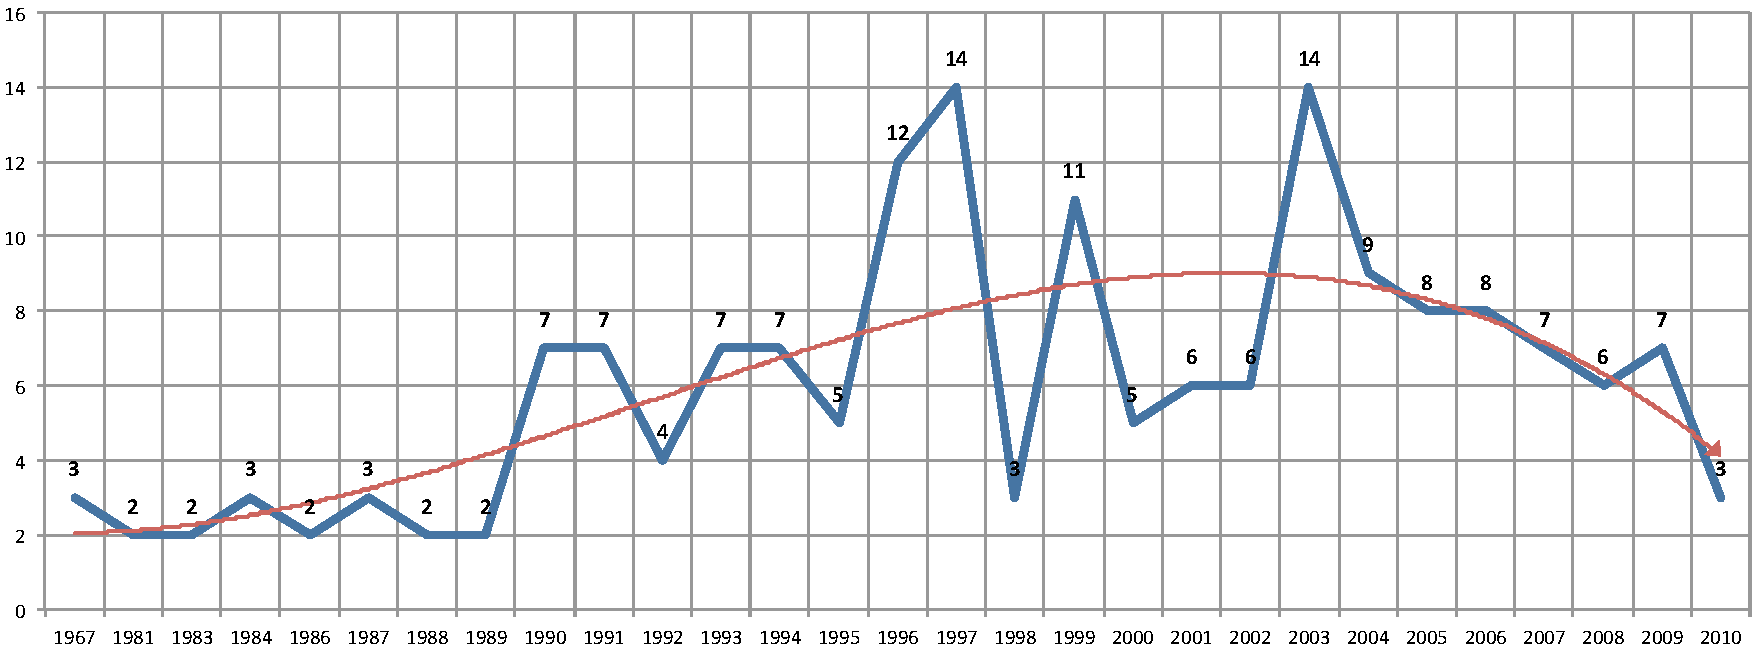
\includegraphics[scale=0.5]{imagens/abntex2-modelo-img-grafico.pdf}
	\legend{\textmd{Fonte: \citeonline[p. 24]{araujo2012}}}
\end{figure}

Todas as figuras ou tabelas inseridas no trabalho, deve ser comentada no texto, e devem ser chamadas pela sua numeração dentro do texto, e não como ``a figura abaixo ou acima''. As figuras e tabela devem ser centralizada com legenda no formato ``Figura x – texto'' ou ``Tabela x – texto'' vindo antes da mesma usando Times 10, negrito, espaçamento 1,5 e centralizada e após a figura ou tabela referenciar a fonte. Segundo a \cite{NBR14724:2011} ``...após a ilustração, na parte inferior, indicar a fonte consultada (elemento obrigatório, mesmo que seja produção do próprio autor), legenda, notas e outras informações necessárias à sua compreensão (se houver). A ilustração deve ser citada no texto e inserida o mais próximo possível do trecho a que se refere.''
\section{Seção que fala sobre algo}\label{sec:fund_sobre_algo}
Escrever algo para referenciar a Tabela \ref{tab:anova_delineamento}.
\begin{table}[htb]
\tiny
\caption{ANOVA pra delineamento em quadrado latino}
\label{tab:anova_delineamento}
\centering
\begin{tabular}{ll p{4.5cm} ll}
    \specialrule{.1em}{.05em}{.05em}
    \textbf{Fontes} & \textbf{g.1}  & \textbf{SQ}  & \textbf{E(SQ)} & F0 \\
    \specialrule{.1em}{.05em}{.05em}
    Tratamento & $(t-1)$  & $SQTratamento = \frac{1}{t}\displaystyle\sum_{j=1}^{t} y_j^2 - \frac{y^{2}}{N}$ &  $\frac{SQ_{Tratamento}}{t-1}$ & $\frac{E(SQ)_{Tratamento}}{E(SQ)_{erro}}$ \\
    %\hline
    Linha & $(t-1)$ & $SQLinha = \frac{1}{t}\displaystyle\sum_{i=1}^{t} y_i^2 - \frac{y^{2}}{N}$  & $\frac{SQ_{Linha}}{t-1}$ & \\
    %\hline
    Coluna & $(t-1)$ & $SQColuna = \frac{1}{t}\displaystyle\sum_{k=1}^{t} y_k^2 - \frac{y^{2}}{N}$ & $\frac{SQ_{Coluna}}{t-1}$ &  \\
    %\hline
    Erro & $(t-1) (t-2)$ & $SQ_{Erro} = SQ_{Total} - SQ_{Linha} - SQ_{Tratamento} - SQ_{Coluna}$ & $\frac{SQ_{Erro}}{(t-2)(t-1)}$ &  \\
    \specialrule{.1em}{.05em}{.05em}
    Total & $t^{2}-1$ & $\displaystyle\sum_{i}\sum_{j}\sum_{k} y_{ijk}^2 - \frac{y^{2}}{N}$ &  &  \\
    %\hline
	
\end{tabular}
\\[8pt]
\fbox{\begin{minipage}{1.5cm}
\textbf{Legenda:}\\
\end{minipage}
\begin{minipage}{12cm}
$g.1 \rightarrow$ Grau de liberdade; $SQ \rightarrow$ Soma dos quadrados; $E(SQ) \rightarrow$ Valor esperado dos quadrados médio; $F_{0} \rightarrow$ Estatística de teste $F$
\end{minipage}
}
\legend{\textmd{Fonte: \citeonline{demery2012}}}
\end{table}

Quando a figura, quadro ou tabela pertencerem ao próprio autor referenciar a fonte como ``Elaborada pelo autor''. Pode-se visualizar essa autorreferência no Quadro \ref{quadro:exemplo}.

\begin{quadro}[htb]
\caption{Exemplo de quadro}\label{quadro:exemplo}
\centering
\begin{tabular}{ccc}
    \specialrule{.1em}{.05em}{.05em}
    \textbf{Situação} & \textbf{mmol/L}  & \textbf{mg/dL} \\
    \hline
    Em jejum e antes das refeições & 7,0 & 126 \\
    Uma hora depois de uma refeição & 10,0 & 180 \\
    Duas horas depois de uma refeição & 8,0 & 144 \\
    Antes de dormir (mínimo) & 6,0 & 108 \\
    \specialrule{.1em}{.05em}{.05em}
\end{tabular}
\legend{\textmd{Fonte: Elaborado pelo autor}}
\end{quadro}


\section{Resumo do capítulo}\label{sec:fund_resumo_cap}
Escrever o resumo do capítulo. Esta seção é obrigatória, porém o título poderá ser modificado como exemplo: considerações finais do capítulo, conclusão do capítulo, etc…


	\chapter{Conclusão}

\begin{flushright}
	\begin{minipage}{14.0cm}
			\setlength{\parindent}{0cm}
			\textit{Neste capítulo apresentam-se as considerações finais sobre o trabalho desenvolvido nesta monografia. Na Seção \ref{sec:consideracoes_finais} estão as considerações finais. Na Seção \ref{sec:contribuicoes_trabalho} descrevem-se as contribuições desta monografia e na Seção \ref{sec:proposta_trabalhos_futuros} algumas propostas para trabalhos futuros. \textbf{(item opcional)}}
	\end{minipage}
\end{flushright}

\section{Considerações finais}\label{sec:consideracoes_finais}
Recomendamos fortemente a utilização das seções apresentadas neste capítulo.

\section{Contribuições deste trabalho}\label{sec:contribuicoes_trabalho}
Escrever as contribuições.

\section{Proposta para trabalhos futuros}\label{sec:proposta_trabalhos_futuros}
Escrever aqui.
\end{capitulos}


% ----------------------------------------------------------
% ELEMENTOS PÓS-TEXTUAIS
% ----------------------------------------------------------
%\postextual

% ----------------------------------------------------------

% ----------------------------------------------------------
% Referências bibliográficas
% ----------------------------------------------------------
\begin{referencias}
	\bibliography{referencias}
\end{referencias}
% ----------------------------------------------------------
% Anexos
% ----------------------------------------------------------

% ---
% Inicia os anexos
% ---
\begin{anexosenv}
	
	% ---
	\chapter{Recursos extras de terceiros}\label{anex:recursos_terceiros}
	% ---
	Os anexos são numerados por letra, como visto acima, e são opcionais. Segundo a \cite{NBR14724:2011}, ``Utilizam-se letras maiúsculas dobradas, na identificação dos apêndices, quando esgotadas as letras do alfabeto''.
	
	\lipsum[30]


\end{anexosenv}

% ----------------------------------------------------------
% Apêndices
% ----------------------------------------------------------

% ---
% Inicia os apêndices
% ---
\begin{apendicesenv}

	% ---
	\chapter{Recursos extras autorais}\label{apen:recursos_autorais}
	% ---
	Os apêndices são numerados por letra, como visto acima, e são opcionais. Segundo a \cite{NBR14724:2011}, ``Utilizam-se letras maiúsculas dobradas, na identificação dos apêndices, quando esgotadas as letras do alfabeto''.
	
	\lipsum[50]

\end{apendicesenv}


\end{document}
